\section{Methods}\label{sec:methods}
\paragraph{Generator.} Stable Diffusion~1.5 \citep{rombach2022ldm} at a pinned revision in fp16, DDIM \citep{song2021ddim} with $\eta=0$ and $T=40$ steps at $512^2$ pixels, empty negative prompt. With text condition $c$ and guidance scale $w$, the noise prediction at step $i$ is the classifier-free combination \citep{ho2022cfg}
\begin{equation}
\hat\varepsilon_i = \varepsilon_\theta(x_i,\varnothing) + w_i\,\big(\varepsilon_\theta(x_i,c)-\varepsilon_\theta(x_i,\varnothing)\big),
\end{equation}
where $w_i$ is constant ($w_i=w$) except under the guidance schedules below. When $w_i=1$ only the conditional branch is evaluated, and the number of network evaluations is counted per image.

\paragraph{Outcomes.} An automatic judge (Section~\ref{sec:evaluation}) scores each image for each constraint $\kappa$ of its prompt: presence (all required objects detected), count (exact), and, conditional on the relevant objects being present, colour binding, left/right relation and relative size (box area of the intended larger object at least $1.5\times$ the other's). Conditional outcomes are undefined, not zero, when an object is missing. The adherence score $F$ of an image is the mean of the outcome families present.

\paragraph{Restart probe.} The latent after $t\in\mathcal{G}=\{6,12,18,24,30,36\}$ completed steps is saved. A branch re-noises it to an earlier step index $j$ with fresh noise $\varepsilon\sim\mathcal{N}(0,I)$ and denoises deterministically to the end at the base's guidance:
\begin{equation}
x'_j=\sqrt{r}\,x_t+\sqrt{1-r}\,\varepsilon,\qquad r=\bar\alpha(j)/\bar\alpha(t),
\end{equation}
with $\bar\alpha(s)$ taken at the scheduler timestep of step $s$. The fixed-jump probe (D8) uses $j=\max(t-8,0)$, whose noise share $1-r$ grows with $t$; the equal-ratio probe (ER30) chooses $j$ so that $r\approx0.30$ at every $t$; a full resample (FULL) restarts from pure noise and serves as a validity control.

\paragraph{Chance-corrected persistence.} For scene $s$ and constraint type $\kappa$, let $A_{\kappa s}(t)$ be the share of (base, branch) pairs with equal outcomes and $A0_{\kappa s}$ the agreement between independent seeds of the \emph{same base prompt, guidance and step count}. Persistence pools scenes as a ratio estimator,
\begin{equation}
C_\kappa(t)=\frac{\sum_s\big[A_{\kappa s}(t)-A0_{\kappa s}\big]}{\sum_s\big[1-A0_{\kappa s}\big]},
\end{equation}
so $C=0$ means no more agreement than an independent sample and $C=1$ means the outcome is fixed. $t_{50}^\kappa$ is the linearly interpolated first crossing of $0.5$; it is left-censored when $C$ already exceeds $0.5$ at $t=6$ and right-censored when it never does. Because the noise share of D8 varies with $t$, absolute $t_{50}$ is relative to the probe; ER30 is the registered sensitivity check.

\paragraph{Prompt-switch probe.} A counterfactual trajectory (colour swap, relation reversal or size swap) is continued from its saved state with the canonical prompt, and
\begin{equation}
C^{\mathrm{switch}}(t)=\frac{\sum_s\big[W_s(t)-W0_s\big]}{\sum_s\big[W1_s-W0_s\big]},
\end{equation}
where $W$ is the share of switched images satisfying the counterfactual constraint and $W0$, $W1$ are that share among canonical and counterfactual images.

\paragraph{Attention stabilisation.} Cross-attention maps of the constraint words are recorded at every step (conditional branch, averaged over heads and over layers within the $16\times16$ and $32\times32$ groups; recording leaves the image unchanged). Per type a signal $a_i$ is formed (noun map, colour-word map, ratio of effective areas, angle between noun centroids, connected components), its velocity $v_i=1-\cos(a_i,a_{i-1})$ (or the absolute change of a scalar), and $t_{\mathrm{stab}}$ is the step at which half of the cumulative path $\sum_i v_i$ has been travelled.

\paragraph{Commitment-Aligned Guidance.} For a prompt with constraint types $K$, the switch step and the schedules are
\begin{equation}
s^\star=\min\!\Big(\big\lceil\max_{\kappa\in K}t_{50,\mathrm{DEV}}^{\kappa}\big\rceil+2,\;T\Big),\qquad
w_i^{\mathrm{A2}}=\begin{cases}w_{hi}&i<s^\star\\ w_{lo}&i\ge s^\star\end{cases},\qquad
w_i^{\mathrm{A4}}=\begin{cases}w_{lo}&i<s^\star\\ w_{lo}+\frac{s^\star(w_{hi}-w_{lo})}{T-s^\star}&i\ge s^\star\end{cases},
\end{equation}
with $w_{hi}=7.5$. A4 has the same mean guidance as A2 in reverse order; A6 applies that mean as a constant; A3 uses a global $s^\star$ from the median DEV $t_{50}$; A1 is constant $7.5$. The frozen design uses $w_{lo}=\wLo$, selected by the DEV quality guard (Section~\ref{sec:resDEV}); Figure~\ref{fig:schedules} shows the exact schedules for the two switch steps that occur on the test split.
\begin{figure}[t]\centering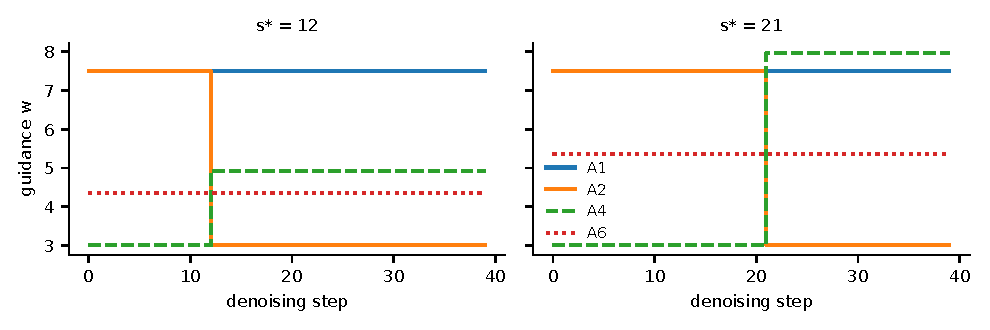
\includegraphics[width=\linewidth]{figures/fig_cag_schedules.pdf}
\caption{Exact guidance schedules of the frozen design (computed by \texttt{src/cag.py}) for $s^\star=12$ and $s^\star=21$ with $w_{lo}=\wLo$: constant CFG (A1), CAG (A2), reversed with equal mean (A4) and constant at A2's mean (A6). A4 is not capped; its maximum guidance is recorded per job.}\label{fig:schedules}\end{figure}

\paragraph{Statistical analysis.} Uncertainty uses a scene-level bootstrap with $10{,}000$ draws and fixed random keys, resampling scenes (not images) so that seeds and branches of a scene stay together; $p$-values are bootstrap tail probabilities. Holm's procedure controls the family-wise error over HA, HD, HE and HF, with a non-estimable hypothesis counting as $p=1$. Identical generations (same prompt text, guidance, steps and seed in one split) are counted once, two canonical scenes with identical text count once, and test prompts whose text also occurs in the development split are excluded from variant-level summaries.

\paragraph{Sensitivity to judge error (exploratory, not registered).} Restart persistence is a statement about agreement between judged outcomes, so judge errors enter both $A$ and $A0$. If each judged outcome is flipped independently with probability $e$ (symmetric, non-differential error), every observed agreement is the affine image $A^{\mathrm{obs}}=(1-2e)^2A+c$ of the true agreement with $c=2e(1-e)$, for branch pairs and seed pairs alike. Substituting into the pooled estimator gives the error-corrected persistence
\begin{equation}\label{eq:err-corr}
C_\kappa^{(e)}(t)=\frac{\sum_s\big[A^{\mathrm{obs}}_{\kappa s}(t)-A0^{\mathrm{obs}}_{\kappa s}\big]}{\sum_s\big[1-c-A0^{\mathrm{obs}}_{\kappa s}\big]},
\end{equation}
which equals the registered $C_\kappa(t)$ at $e=0$. Error makes $C$ shrink towards zero by an amount that depends on $A0$, which differs between guidance scales. The model assumes errors independent across images; a detector's errors are usually content-dependent (the same hard object is missed in every seed), which can move agreement in either direction and is not captured. We therefore use Eq.~\eqref{eq:err-corr} as a stress test of how much judge noise a conclusion tolerates, not as a correction of the estimate, and evaluate $e\in\{0.05,0.10\}$ and $e=1-\text{(audited presence accuracy)}$.
